\chapter{Verifica}\label{chp:verifica}
In fase di verifica si è fatto uso della funzione \texttt{print\_update(\dots)} per monitorare l'avanzamento della simulazione \textit{step-by-step}, con l'obiettivo di controllare che l'evoluzione dello stato del sistema avvenisse fedelmente ai modelli precedentemente descritti (capp. \ref{chp:modello-concettuale}, \ref{chp:modello-specifiche}, \ref{chp:modello-computazionale}).

Gli screenshot riportati nelle figure che seguiranno in questo capitolo (figg. \ref{fig:verifica-1} e \ref{fig:verifica-2}) sono stati tutti quanti realizzati fissando come seed iniziale \texttt{9}.

\section{Controlli di consistenza sullo scheduler}
I controlli di consistenza effettuati sullo scheduler sono di seguito analizzati:
\begin{itemize}
\item In figura \ref{fig:verifica-1a} è mostrata una verifica di come, in assenza di ticket di tipo \sr{} da processare (evidenziato in {\color{verify_blue}blu}), il server dedicato si comporta come se fosse generale, infatti elabora una richiesta \pp{} \textsl{BancoPosta} (evidenziato in {\color{verify_red}rosso}).
\item In figura \ref{fig:verifica-1b} è mostrata una verifica di come, in presenza di ticket di tipo \sr{} da processare (evidenziato in {\color{verify_blue}blu}), il server dedicato ignora la coda \pp{} \textsl{Standard} ed elabora una richiesta \sr{} \textsl{BancoPosta} (evidenziato in {\color{verify_red}rosso}).
\item In figura \ref{fig:verifica-1c} è mostrata una verifica di come un server possa essere \texttt{IDLE} (evidenziato in {\color{verify_red}rosso}) se e soltanto se non sono presenti richieste pendenti che è in grado di processare (evidenziato in {\color{verify_blue}blu}).
\item In figura \ref{fig:verifica-1d} è mostrata una verifica di come, in presenza di più code non vuote (evidenziato in {\color{verify_blue}blu}), il server dà priorità al cliente appartenente alla classe \uo{} \textsl{Standard} piuttosto che all'altro \pp{} \textsl{Standard} (evidenziato in {\color{verify_red}rosso}).
\end{itemize}

\begin{figure}[ht]
\centering
\begin{subfigure}[b]{0.475\textwidth}
\centering
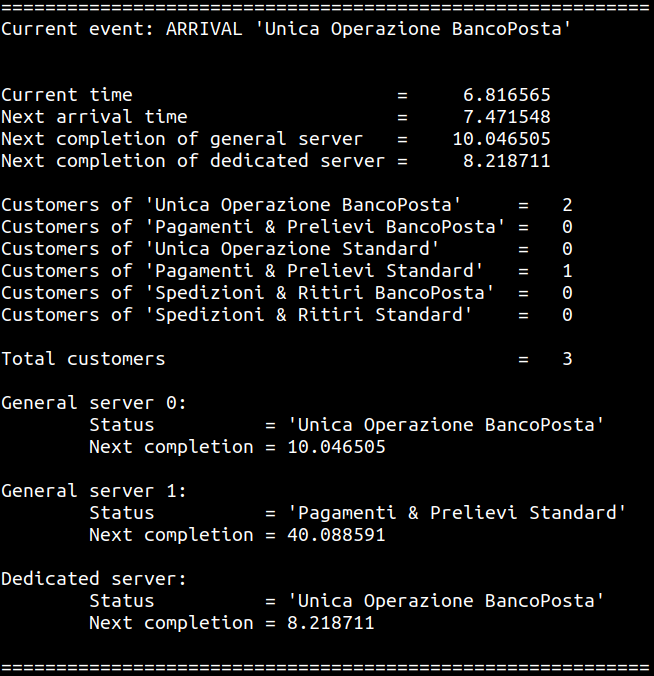
\includegraphics[width=\textwidth]{screenshots/original/ded_server_changes_behaviour}
\caption{Cambio del comportamento del server dedicato}    
\label{fig:verifica-1a}
\end{subfigure}
\hfill    
\begin{subfigure}[b]{0.475\textwidth}  
\centering 
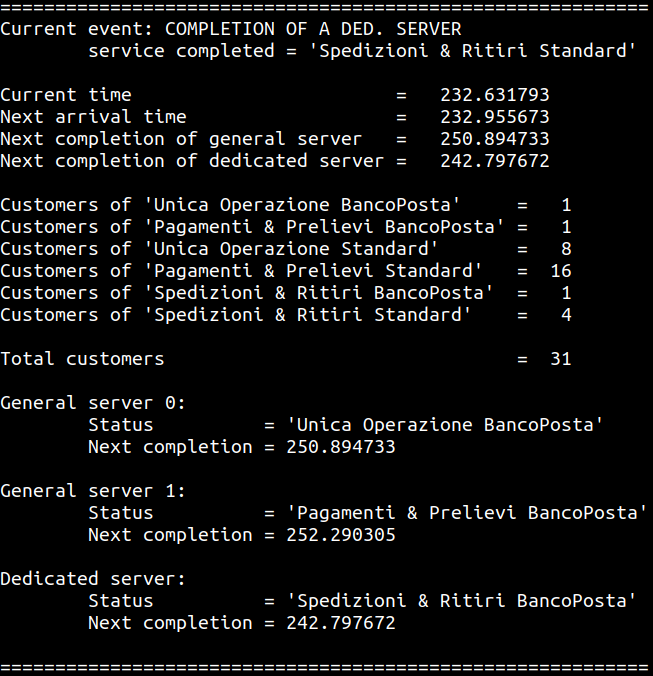
\includegraphics[width=\textwidth]{screenshots/original/ded_server_priority_sched}
\caption{Schedulazione sul server dedicato}    
\label{fig:verifica-1b}
\end{subfigure}


\vskip\baselineskip

\begin{subfigure}[b]{0.475\textwidth}   
\centering 
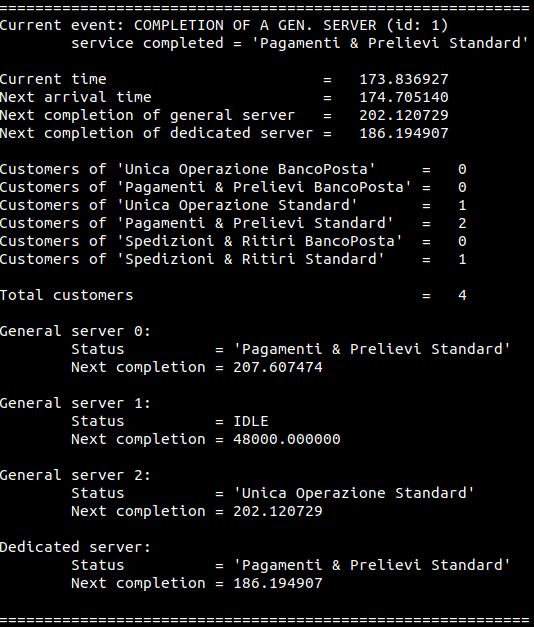
\includegraphics[width=\textwidth]{screenshots/original/gen_servers_no_SR}
\caption{I server generali non processano \sr{}}   
\label{fig:verifica-1c}
\end{subfigure}
\hfill
\begin{subfigure}[b]{0.475\textwidth}   
\centering 
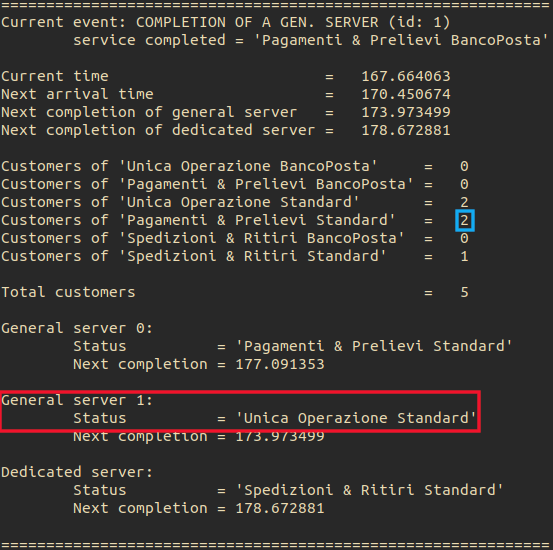
\includegraphics[width=\textwidth]{screenshots/original/gen_servers_priority_sched}
\caption{Schedulazione su un server generale}    
\label{fig:verifica-1d}
\end{subfigure}
\caption{Screenshots della simulazione per la fase di verifica}
\label{fig:verifica-1}
\end{figure}

\section{Controlli di consistenza sulle statistiche di output}
Di seguito vengono effettuati i controlli di consistenza sulle statistiche di output:
\begin{itemize}
\item Per le statistiche job-averaged, per definizione, si ha:
\begin{equation}
\bar{d} = \bar{w} - \bar{s}
\end{equation}
Dalla figura \ref{fig:verifica-2} è facile osservare che questa relazione sia rispettata. Ad esempio, per la classe d'utenza \uo{} \textsl{BancoPosta} vale che $\mathtt{8.74 - 6.12 = 2.62 \simeq 2.63}$.
\item Per le statistiche time-averaged, per definizione, si ha:
\begin{equation}
\bar{q} = \bar{l} - \bar{y}
\end{equation}
Dalla figura \ref{fig:verifica-2} è facile osservare che questa relazione sia rispettata. Ad esempio, per la classe d'utenza \uo{} \textsl{BancoPosta} vale che $\mathtt{0.28 - 0.08 = 0.20}$.
\item Dalla teoria è noto che:
\begin{equation}
\begin{array}{c c c}
\bar{l} = \frac{n}{c_n} \cdot \bar{w}, & \bar{q} = \frac{n}{c_n} \cdot \bar{d}, & \bar{y} = \frac{n}{c_n} \cdot \bar{s} 
\end{array}
\end{equation}
Dalla figura \ref{fig:verifica-2} è facile osservare che questa relazione sia rispettata. Ad esempio, per la classe d'utenza \pp{} \textsl{Standard} vale che $\mathtt{\frac{32}{531.87} \cdot 17.00 = 1.02281 \simeq 1.02}$.
\end{itemize}

\begin{figure}[ht]  
\centering 
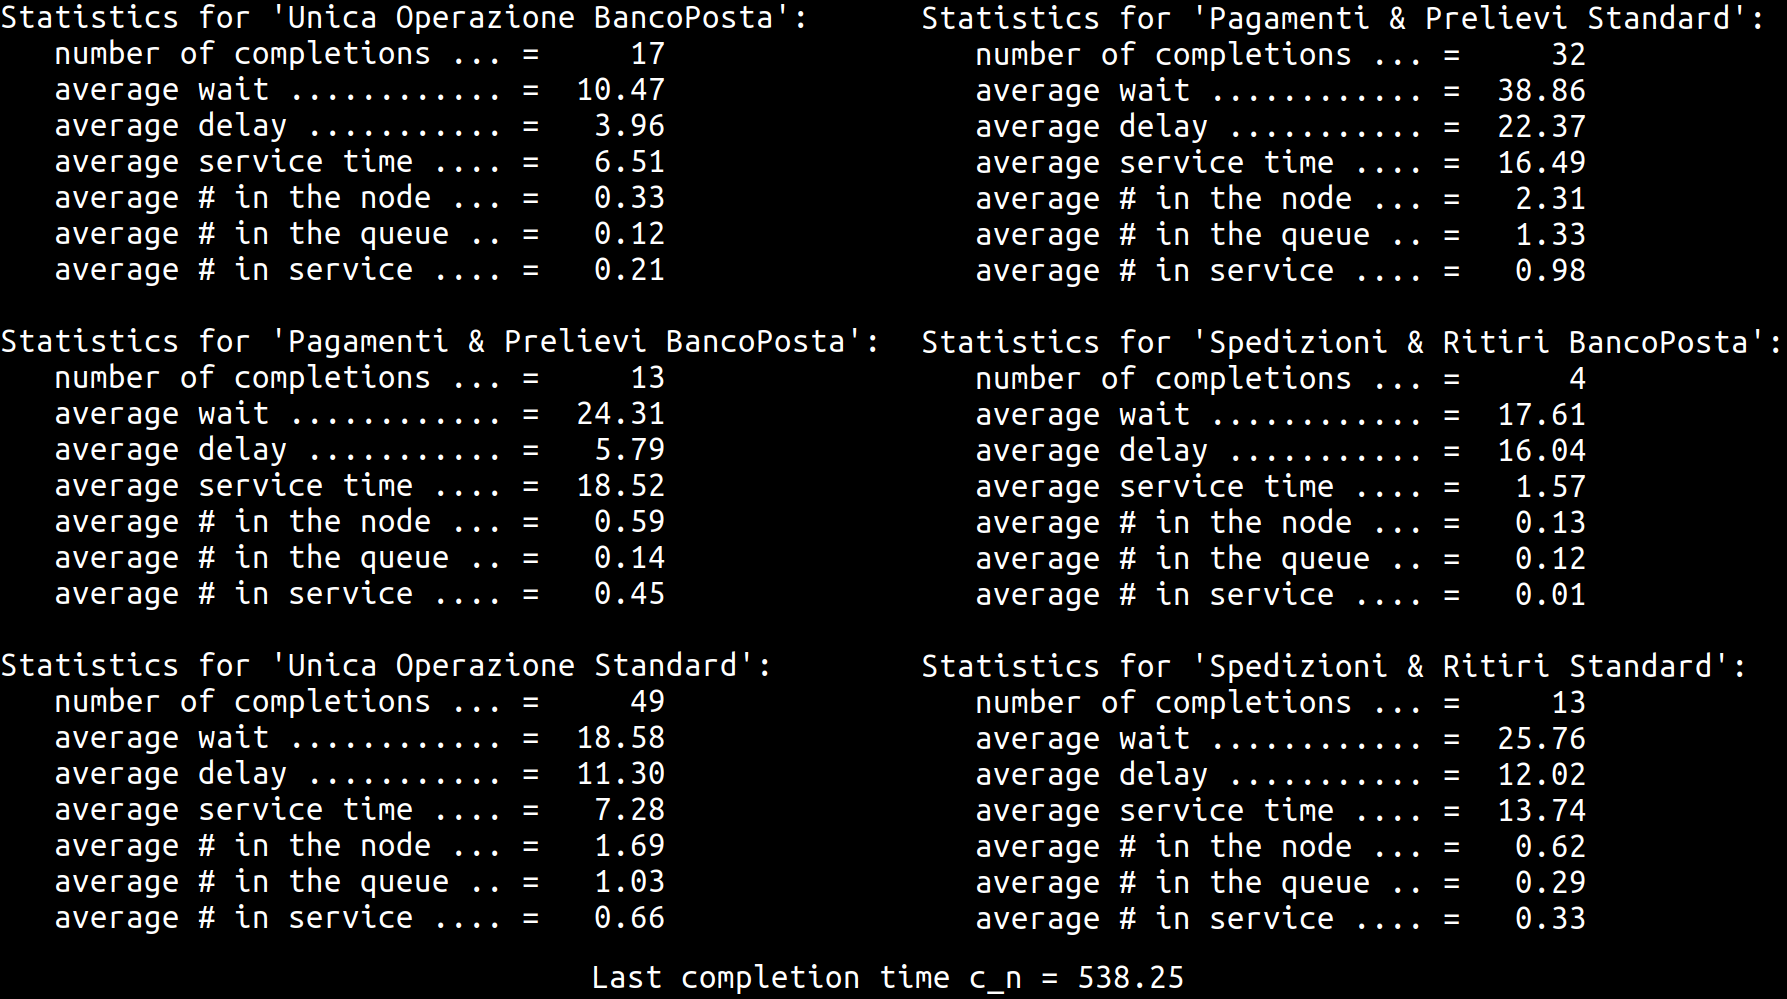
\includegraphics[width=\textwidth]{screenshots/original/statistics}
\caption{Statistiche per ciascuna classe di utenza computate su un singolo run}   
\label{fig:verifica-2}
\end{figure}

